
\documentclass[a4paper]{article}
\usepackage{pslatex}
\usepackage[T1]{fontenc}
\usepackage[utf8x]{inputenc}
\setlength\parskip{\medskipamount}
\setlength\parindent{0pt}
\usepackage{graphicx}
\usepackage{amssymb}
%\usepackage{hyperref}

\usepackage{multicol}

\makeatletter

\providecommand{\boldsymbol}[1]{\mbox{\boldmath $#1$}}
\newcommand{\ASL}			{ASL}
\newcommand{\OSC}[1]		{\texttt{#1}}
\newcommand{\lra}			{$\leftrightarrow$}
\newcommand{\seg}[1]		{Seg(#1)}

\setlength{\parskip}{1mm}

\makeatother

\begin{document}

\title{FaustLive - Specification \\ v.1.2}

\author{Grame, Centre National de Création Musicale\\
{\small <research@grame.fr>} \\
\vspace{2mm}
[ANR-12-CORD- 0009] and [ANR-13-BS02-0008]
}

\maketitle

\topskip0pt

\newpage
\tableofcontents

\newpage
\section{General Considerations}

\subsection{FaustLive}
FaustLive is an advanced self-contained prototyping environment for the Faust programming language with an ultra-short edit-compile-run cycle. Thanks to its fully embedded compilation chain, FaustLive is simple to install and doesn't require any external compiler, development toolchain or SDK to run. FaustLive is the ideal tool for fast prototyping. Faust programs can be compiled and run on the fly by simple drag and drop. They can even be edited and recompiled while running without sound interruption or Jack disconnection. \\
\\
FaustLive is based on QT. Most classes are a reimplementation of QObjects. 
To know more about these base-objects, see QT documentation : http://qt-project.org/doc/qt-5/classes.html

\subsection{Code Structure}

The structure of FaustLive is based on three main classes : FLApp, FLWindow and FLSessionManager.

\begin{itemize}
\item FLApp is a reimplementation of QApplication. Its role is to be a communication center between the menus, dialogs, windows, etc. 

\item FLWindow reimplements QMainWindow. Its role is to contain the DSP, its interface(s) and react to the window's menus/actions/...

\item FLSessionManager is a simple QObject. Its role is to be the compilation center and maintain the hierarchy of the current session. 

\end{itemize}

Many of the dialogs and internal structure classes are singletons to share their information with one shared access point. 

%%%%%%%%%%%%%%%%%FAUSTLIVE APP%%%%%%%%%%%%%%%%%%%
\section{FLApp}
 
FLApp reimplements QApplication. For that matter, it contains the main event loop, where all events from the window system and other sources are processed and dispatched. It also handles the application's initialization (some singletons have to be initialized by FLApp) and finalization.

\subsection{Menus}

The menus are handled differently, depending on the platform. \\
On OSX, the menu of the application appears in the system external menu-bar. Depending on the front window, the specific menus will show. \\
On Windows and Linux, each window of the application has its own menu-bar. There is no general menu-bar. That is why, when the last window is closed, the application quits. \\

While some actions are specific to the windows (edit, export, ...), others have to be treated by the application (new, open, ...). The application-related menus and actions have to be created by the application to be connected to its SLOT. 

So, FLApp contains the following functions, for menu creation :
\begin{itemize}
\item create\_FileMenu() : QMenu* 
\item create\_ExampleMenu() : QMenu*
\item create\_RecentFileMenu() : QMenu*
\item create\_NavigateMenu() : QMenu*
\item create\_HelpMenu() : QMenu*
\end{itemize}

In order to appear in the window menu-bar, the list of menus is then passed to the window when it is created.

\subsection{Create FLWindow}

FLWindows are characterized by their settings. So that FLApp has to choose them before creating a new FLWindow. Their are different ways to get the settings :

\begin{itemize}
\item Create new settings
\item Recall existing settings
\item Copy existing settings
\end{itemize}

In case the settings are new, some parameters have to be initialized like the index of the window (smallest not currently used), the position of the window on screen, ...

Once the Window is created, it has to be initialized with the Faust source (see createWindow).

\section{Menus and Dialogs}

\subsection{FLErrorWindow}

FLErrorWindow reimplements QMainWindow. Its role is to displays all errors occurring in the program.
FLErrorWindow is a singleton.

\subsection{FLMessageWindow}

FLMessageWindow reimplements QDialog. Its role is to displays messages printed by the program, like (Compiling DSP..., etc)
FLMessageWindow is a singleton.

\subsection{FLHelpDialog}

FLHelpDialog reimplements QDialog. Its role is to display the help menu, for the user to get information of FaustLive uses. 

\subsection{FLPreferenceWindow}

FLPreferenceWindow reimplements QMainWindow. Its role is to display the preferences of FaustLive and handle the changes of settings. 

\subsection{FLPresentationWindow}

FLPresentationWindow reimplements QMainWindow. Its role is to display the presentation menu.

\subsection{FLExportManager}

FLExportManager contains two classes classes describing the two dialogs used in the export process. The first dialog presents all the targets available. The second one shows the steps of the evolution of the export.

%%%%%%%%%%%%%%%%%WINDOW%%%%%%%%%%%%%%%%%
\section{FLWindow}

FLWindow reimplements QMainwindow. Its role is to display the DSPs QTinterface and to wrap it with its specific toolbars and menus to access some more interactive features. 

\subsection{Interface-related functions}

One FLWindow contains multiple types of interface, from which some are optional. 

\begin{itemize}
\item QTGUI : interface displayed in FLWindow
\item FUI : interface saving the interface parameters
\item HTTPUI : interface handling the HTTP protocol for remote control
\item OSCUI : interface handling the OSC protocol for remote control 
\end{itemize}

Each type of interface has its set of function to run in FLWindow (allocate, buildUserInterface, run, delete);

\subsection{Audio-related functions}

To create an audio client, corresponding to the DSP, running in FLWindow, FLWindow has to create an audio manager through audioclient (only class able to create the right audioManager : see AUDIO).

\begin{itemize}
\item init\_audioClient : init audioManger. The type of manager is not known in FLWindow, it is the AudioCreator that returns 
\item setDSP : setDSP 
\item audioShutDown
\item start/stop\_Audio

\end{itemize}
\subsection{ToolBar-related functions}

\begin{itemize}
\item set\_ToolBar : the toolbar has to be created and its signals connected to the window SLOT
\item resizingSmall/Big : close/open toolbar
\item setWindowsOptions : the options contained in FLToolBar can be modified outside of the toolbar (OSCUI ports for example when already used), so they have to be synchronized
\item modifiedOptions : reaction to the modification of the compilation options from toolbar
\item generateAuxFiles : reaction to the modification of the automatic export options from toolbar
\item switchOsc : enable/disable OSC interface
\item updateOSCInterface : update OSC interface with new port options
\item switchHttp : enable/disable HTTP interface
\item switchRelease : enable/disable factory publication
\item switchRemoteControl : enable/disable remote control interface
\end{itemize}

\subsection{StatusBar-related functions}

\begin{itemize}
\item set\_StatusBar : the status bar has to be created
\item redirectSwitch : update the window with new machine options
\end{itemize}

\subsection{Menu-related functions}



\subsection{Drag and Drop related functions}

A window has to be set up for Drag and Drop, so that setAcceptDrops is set to "true" in FLWindow constructor.

\begin{itemize}
\item dragEnterEvent : describes the filters 
\item dragLeaveEvent : 
\item dropEvent
\item pressEvent
\item eventFilter
\end{itemize}

%%%%%%%%%%%%%%%%%SESSION MANAGER%%%%%%%%%%%%%%%%%
\section{FLSessionManager}

FLSessionManager is a singleton.\\

The role of FLSessionManager is to be the link with libfaust and libfaustremote, to compile the DSPs. Moreover, it has the purpose to maintain the hierarchy of the current session and be able to save/recall sessions and snapshots. 

\subsection{Current Session Hierarchy}

The current session is composed of : 
\begin{itemize}
\item Settings.ini : file containing the saved settings as described in FLSettings
\item Examples : folder containing a copy of the example files of the faust distribution
\item Libs : folder containing a copy of the libraries of the faust distribution
\item Windows : folder containing the window-specific folders FLW-i, containing :
	\begin{itemize}
		\item Settings.ini : the window specific settings as described in FLWinSettings
		\item Graphics.rc : file saving the graphical parameters of the last DSP contained in the window
		\item Connections.jc : file saving the last known Jack connections of the window
		\item SHAKey.dsp* : copy of the faust code of the last DSP contained in the window (in case the original file is deleted or modified outside of FaustLive execution)
	\end{itemize}
\item SHAFolder : folder containing the DSP-specific folders, containing : 
	\begin{itemize}
		\item SHAKey* : LLVM intermediate representation of the DSP, to accelerate compilation when the same DSP is reused.
		\item SHAKey.dsp*: copy of the Faust code corresponding to this SHAKey
		\item SHAKey-svg* : folder containing the svg diagram resources
	\end{itemize}
\end{itemize}

*To establish an injection between a DSP and its saving files, the SHA-1 hash function is used. This SHAKey is calculated from the faust code before compilation and its compilation options. That way, one code, compiled with different options is always saved. 

\subsection{DSP compilation}

To compile a DSP, there are two steps :
\begin{itemize}
\item create a factory (builds the protoype of a the DSP class)
\item create an instance of the factory (equivalent of a 'new class" in C++)
\end{itemize}

Because FaustLive enables remote processing, the factories and instances it creates can whether be local (llvm\_dsp\_factory / llvm-dsp ) through libfaust or remote (remote\_dsp\_factory / remote-dsp) through libfaustremote. \\

The goal of FLSession Manager is to be the only class that deals with remote\_dsp\_factory, llvm\_dsp\_factory, remote-dsp, llvm-dsp, ...

The classes that will need compilation will only receive a pointer to a dsp, without knowing its type. \\

Still, the two steps cannot be united in the same function, because some audio initialization is needed between the two steps (for the remote case where the sample rate and buffer size are needed to create the instance and only available once the factory is created...).

In conclusion, to create a dsp, there are those two functions :
\begin{itemize}
\item createFactory(const QString\& source, QString\& errorMsg, FLWinSettings* settings = NULL) \\ returns QPair<QString, void*> ;
\item createDSP(QPair<QString, void*> factorySetts, const QString\& source, QString\& errorMsg, FLWinSettings* settings = NULL, RemoteDSPErrorCallback error\_callback = NULL, void* error\_callback\_arg = NULL) \\ returns dsp*;
\end{itemize}

\subsubsection{create Factory}

The creation of the factory is done from a file, saved in the current session and named after the SHAKey (see footnote (1)). So the first step of factory creation is to get the faust content to compile (from the source )


\subsubsection{create Instance}

\subsection{Session/Snapshot restoration}

%%%%%%%%%%%%%%%%%SETTING STRUCTURE%%%%%%%%%%%%%%%%
\section{Setting Management}

%%%%%%%%%%%%%%%%%GENERAL SETTINGS%%%%%%%%%%%%%%%%%
\subsection{FLSettings}

FLSettings is a singleton. 
To save settings, the class FLSettings reimplements QSettings. A hierarchy, presented {Figure \ref{fig:FLSettings}, allows us to access the settings easily. \\

The setting file is saved at the root of the current session (/Users/you/.FaustLiveCurrentSession-version).
 
\begin{figure}[!h]
\begin{center}
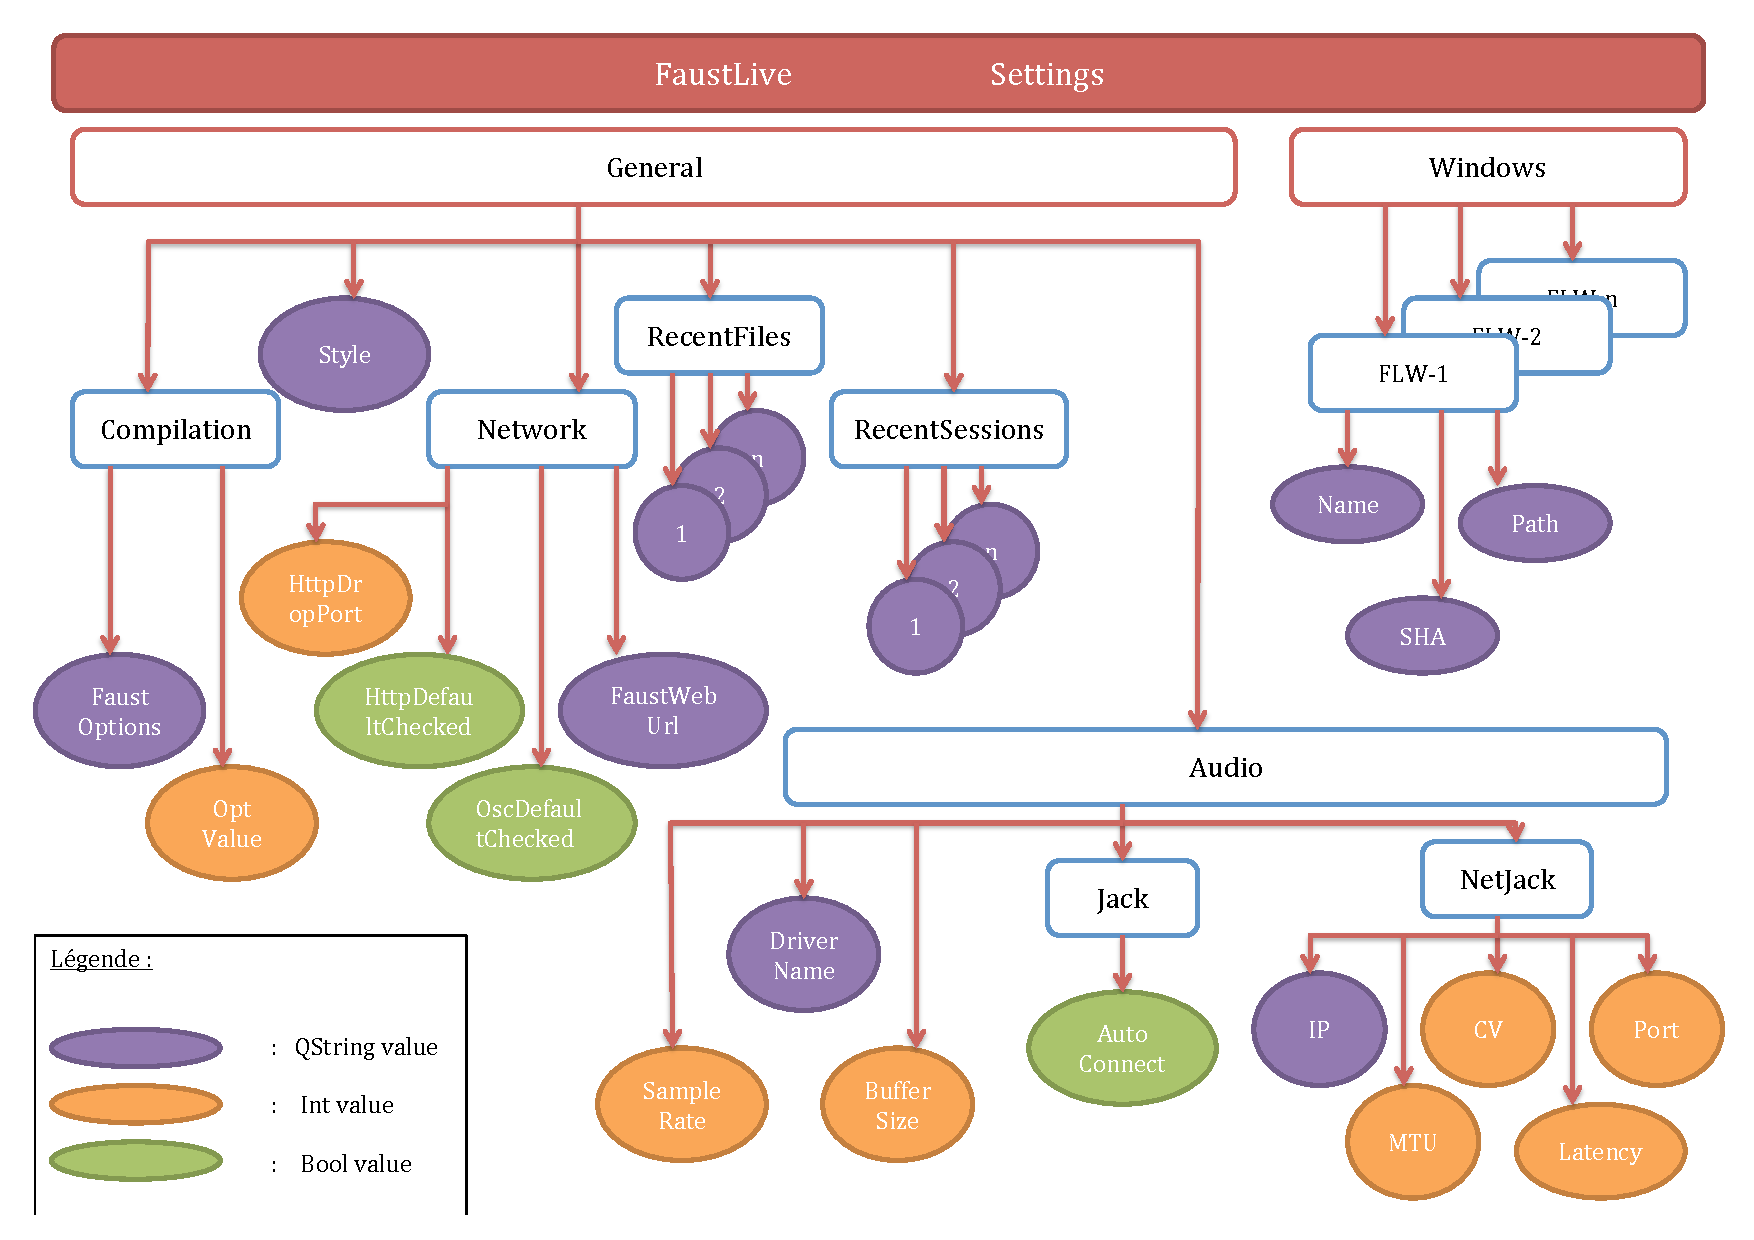
\includegraphics[width=\columnwidth]{images/FLSettings}
\caption{FLSettings structure}
\label{fig:FLSettings}
\end{center}
\end{figure}
 
For example, the value is accessible like this :\\
\textit{int httpPort = FLSettings::\_Instance()->value("General/Network/HttpDropPort", defaultValue);}

%%%%%%%%%%%%%%%%%WINDOW SETTINGS%%%%%%%%%%%%%%%%%
\subsection{FLWinSettings}

FLWinSettings reimplements QSettings. But, this class is not a singleton, each FLWindow is associated to a FLWinSettings. 

\begin{figure}[!h]
\begin{center}
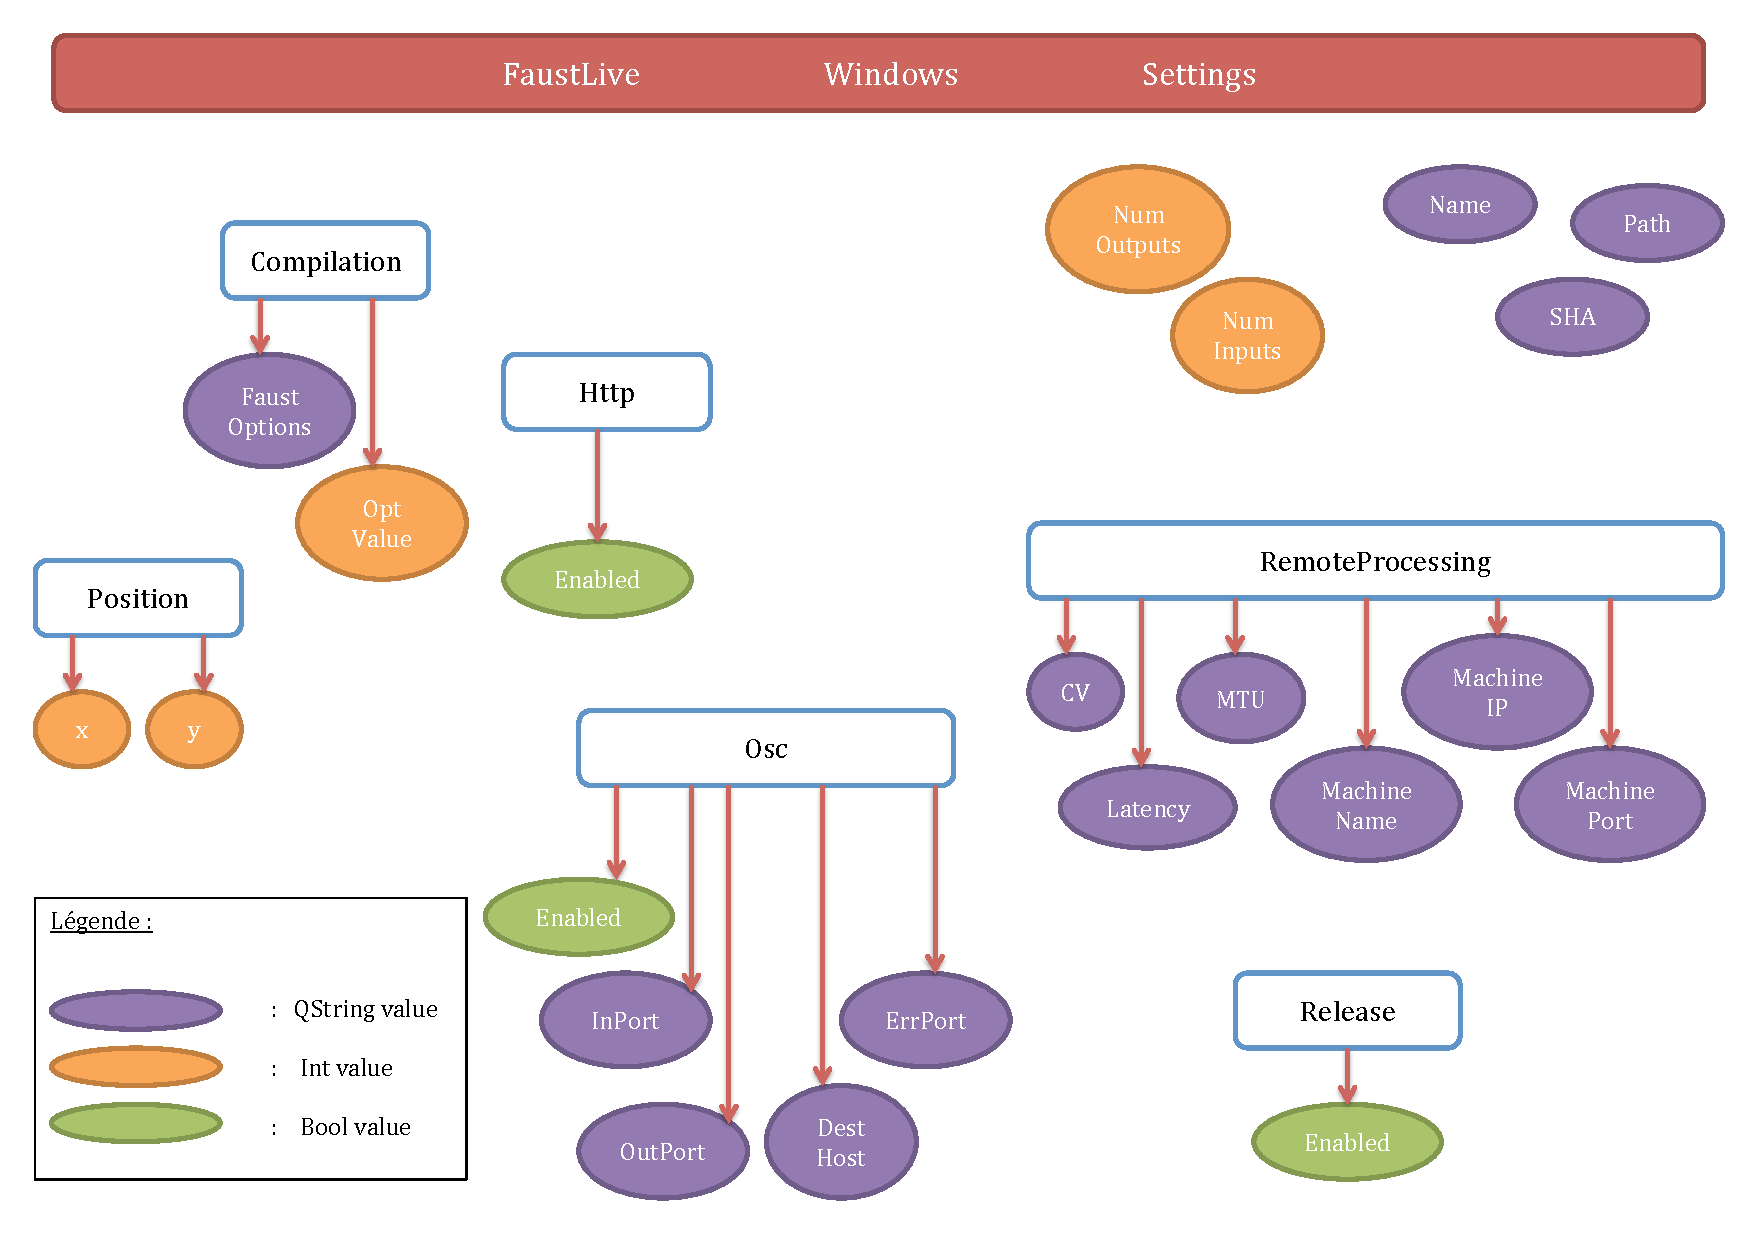
\includegraphics[width=\columnwidth]{images/FLWinSettings}
\caption{FLWinSettings structure}
\label{fig:FLWinSettings}
\end{center}
\end{figure}


For example, the value is accesible like this :\\
\textit{int oscInPort = fSettings->value("Osc/InPort", defaultValue);} \\

 *** The added feature of FLWinSettings, compared to QSettings, is to synchronize three parameters of the window with the general settings. That way, Name, SHA and Path are also accessible from the general settings. This feature is really usefull for snaspshot and session restoration, to have a global vision of the existing windows.

%%%%%%%%%%%%%%%%%AUDIO STRUCTURE%%%%%%%%%%%%%%%%%
\section{Audio}

There are two aspects that have to be managed in the audio section. First what kind of driver is used/usable to take care of the audio rendering ? Then, how do we want to manage the transition between two DSPs relaying in the same window. To respond to that particuliar problem, it was chosen to fade out the out-going DSP while fading in the in-coming DSP. That way, a smooth transition is ensured. 

\subsection{Audio drivers used by FaustLive}
 
Depending on the operating system and the compiling options, it is possible to embed different audio architectures in FaustLive.
Default drivers are :
\begin{itemize}
\item Coreaudio on OSX
\item Jack on Linux
\item Portaudio on Windows
\end{itemize}

Then Jack, NetJack and PortAudio can be added with make options : JACK=1 NETJACK=1 PORTAUDIO=1.

\subsection{Code Organisation}

The general structure of the code is based on the "abstract factory" pattern. That way, the class "AudioCreator" is the only class knowing which type of driver is used, creating the driver-specific factory.  \\

The abstract factory contains the following pure virtual functions :
\begin{itemize}
\item createAudioSettings(QGroupBox* parent)
\item createAudioManager(AudioShutDownCallaback, void* arg)
\end{itemize}

Then each audio driver has its own set of classes :
\begin{itemize}
\item audioFactory : creates the driver-specific elements (audioSettings and audioManager)
\item audioSettings : contains the settings needed by the driver and their graphical representation
\item audioFader : mixes the audio and crossfade features
\item audioManager : manipulates the audio faders and manage their crossfades 
\end{itemize}

\subsection{Crossfade implementation}

The constraint is to smooth the transition between two relaying DSP in a situation of drag and drop or source edition. If a DSP is not changed, the transition should not be hearable. \\
Now, to implement this, some basic functions are common to all implementations and are divided into two classes :
\begin{itemize}
\item AudioFader\_Interface : containing the basic instructions needed by the client to launch a crossfade and know when it stopped. 
\item AudioFader\_Implementation : containing the calculation functions of the crossfade.
\end{itemize}

In order to add the crossfade feature to the audio clients, a reimplementation of the audio classes was made.
The doble inheritance of these "audioFader" permits to mix the audio features and the crossfade features. \\
The separation between interface and implementation sometimes had to be made because some audio classes (like coreaudio-dsp) already made the difference (coreaudio/TCoreAudioRenderer). 

\subsection{AudioManager}

There are two approach of the audio manager structure :
\begin{itemize}
\item the one managing one current client and fading the DSPs in one only client
\item the one managing one current client and creating a second one fading in to replace the current one
\end{itemize}

\subsection{How to add a new audio architecture}

To add a new type of driver audio in FaustLive, the first step is to implement the driver-specific set of classes :
\begin{itemize}
\item audioFactory
\item audioSettings
\item audioManager
\item audioFader
\end{itemize}

Then, some elements have to be added to the class "AudioCreator" : 
\begin{itemize}
\item add the new architecture to the enum "AudioArchitecture"
\item add a new item in the comboBox "fAudioArchitecture"
\item add a new case in createFactory
\end{itemize}

Finally, FaustLive.pro has to be modified (for each platform compatible with the new driver), in order to add the librairies (through conditional compilation or not).

%%%%%%%%%%%%%%%%%REMOTE INTERFACES%%%%%%%%%%%%%%%%%
\section{Remote Interfaces}
\subsection{HTTP interface}
\subsection{OSC interface}
\subsection{Remote interface}

%%%%%%%%%%%%%%%%%REMOTE INTERFACES%%%%%%%%%%%%%%%%%
\section{FLComponentWindow}

The component window is a feature allowing the user to compose DSPs in a parallel/sequence/recursive way to create a new DSP. 
As in the FLWindow, it is possible to drop files and urls, so that you can combine elements from the web with local DSPs to create a new one. \\ 

The resulting DSP is a sequence of "stereoized parallel DSPs" : DSPs are first composed in parallel, then stereoized (see stereoize in music.lib) and finally put in sequence. \\

\subsection{Layout Optimization}

An "optimized" layout for the resulting DSP is calculated, taking as goal to reduce the surface of the interface. In order to do that, a binary tree of items is created. In this tree there are three types of elements : 
\begin{itemize}
\item leaf nodes : containing the real faust element
\item vertical containers, putting in a vertical group it's two sub-nodes
\item horizontal containers, putting in a horizontal group it's two sub-nodes. 
\end{itemize}

Each element of the tree has a function render, so that called on the root node, the whole layout is calculated.

%%%%%%%%%%%%%%%%%DISTRIBUTION STRUCTURE%%%%%%%%%%%%%%%%%
\section{Distribution Structure}

--> Build Folder with targets
--> 

\subsection{Create a new distribution}

--> 







\end{document}




